\chapter{The HADES detector}
\label{chapter:detector}
The \textbf{H}igh \textbf{A}cceptance \textbf{D}i-\textbf{E}lectron \textbf{S}pectrometer (HADES) \cite{Agakishiev:2009am} is located at the GSI Helmholtzzentrum f{\"u}r Schwerionenforschung. The HADES detector was designed for various measurements with the especial emphasis on di-electron spectroscopy. Thanks to versatility of the SIS18 (German: \textbf{S}chwer\textbf{I}onen\textbf{S}ynchrotron) accelerator and a secondary pion beam facility, various kind of experiments can be conducted: starting from pion scattering on proton or nucleus targets, through proton-proton and proton-nucleus reactions, up to the heavy ion collisions. Up to now following experiments have been performed: C+C@2~GeV/u, p+p@2.2~GeV, Ca+KCl@2~GeV/u, C+C@2~GeV, Ar+KCl@1.765~GeV/u, p+p@1.25~GeV, p+p@3.5~GeV, d+p@1.25~GeV/u, p+Nb@3.5~GeV/u, Au+Au@1.23~GeV/u, $\pim$+$\mathrm{C_2H_4}$@1.7~GeV/u, Ag+Ag@1.58~GeV/u.

The detector provides almost full azimuntal angular coverage, whereas the acceptance in the polar angle used to rate from 18$^{\circ}$  to 80$^{\circ}$. A current upgrade extands the detector acceptance for forwards angles, for more detaisl see \ref{subsec:FwDet}. Two sets of toroidal \textbf{M}ulti-wire \textbf{D}rift \textbf{C}hambers (MDC) together with a superconducting toroid magnet allow for momentum measurements with $\frac{dp}{p} \approx 2-3\%$ and particle identification (PID) via energy loss measurement. The PID is further enhanced by high resolution \textbf{T}ime \textbf{O}f \textbf{F}light (TOF) detectors ($\sigma \approx 80$ ps) and a hadron-blind \textbf{R}ing \textbf{I}maging \textbf{CH}erenkov (RICH) detector. A combined information form the detectors allow for efficient p/$\pi$/K/e separation over broad momentum range. Even though it isn't a $4 \pi$ detector, thanks to its geometry it has acceptance around 40\% for pions produced in elementary collisions at energfys provided by SIS18 detector. 
\section{Tracking system}
The HADES tracking system bases on four sets of a drift chambers. Two before and two after a magnetic field. First set is called inner MDC, the second outer MDC. Each single drift chamber has a trapezoidal shape and consist of 13 layers of wires. They create 6 layers of a drift cells. A shape of the sells and the wires dencity was optimalized to get the best momentum resolutions.

Inbetween iner- and outer-MDC the \textbf{I}ron\textbf{L}ess \textbf{S}uperconducting Electron (ILSE) magen is located. It consist of six superconducting coils, which produce a toroidal magnetic field of 3.6 T inside the coils. The operational current can variy from 0 to 3500 A. 

The magnetic field produced by ILSE bends particles' tracks what allows for a momentum reconstruction. Tracks reconstruced in iner- and outer-MDCs have to be matched together. A deticated algorithm for this purpuse was developed by HADES collaboration. 

\section{META detectors}
A META detector during pp and pNb experiments consisted of two time of flight detectors: TOF and TOFino


\section{RICH detector}
The \textbf{R}ing \textbf{I}maging \textbf{CH}erenkov detector is the main tool for $\epem$ identyfication for the HADES. The detector active area surrounds target area and it is filled by a radiator gas ($\mathrm{C}_4 \mathrm{F}_{10}$). A refractive index gives a thrashold speed for a Cherenkov radiation production $\gamma_{thr} =18$. For projectile energys delivered by the SIS18 only particles able to exceed the threshold are electrons end positons. Passing across the radiator they produce a cone of a cherenkov light. Then, the light is reflected by a spherical mirror and detected by a pad plane located upstream a beam. The detector is completelly \``hadronic blind\'' what means that no hadron can give an signal in it. In 2019 the RICH was updated by a new readout system, described more detailed in next section. 
\begin{figure}
  \centering
  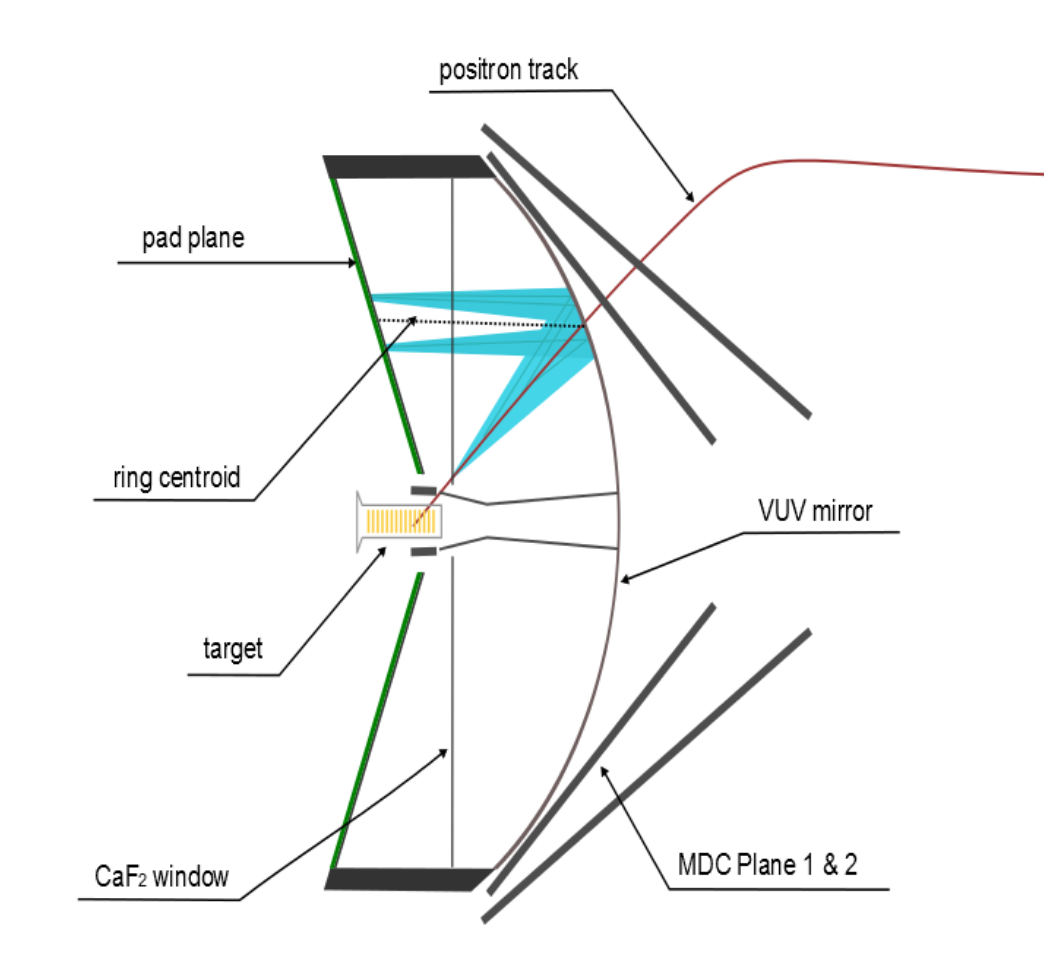
\includegraphics[width=0.6 \linewidth]{Chapter_detector/RICH.png}
  \caption{The \cs of the RICH detector.}
\end{figure}
\section{The HADES upgrades}

\subsection{The Forward Detector}
\label{subsec:FwDet}
In many studies especially devoted to hyperons' decays the forward angles play very important role. The hades detector for a quite long time did not have a possibility to register particles 
\subsection{RICH update}

\subsection{Electromagnetic calorimeter}

\label{chapter:HADES_upgrades}